\subsection{Data processing}
	As a result of the calculations, which took about a month, $.dat$ files were obtained. Each of these data arrays corresponds to a certain time step. For post processing and plotting based on them, the built-in ANSYS CFD-Post tool was used. To analyze the effect of vortex generators on local friction and transfer, different sections were used in different parts of the channel. Some of them are shown on the figure \ref{fig:planesforanalysis}. 
	\begin{figure}[H]
		\centering
		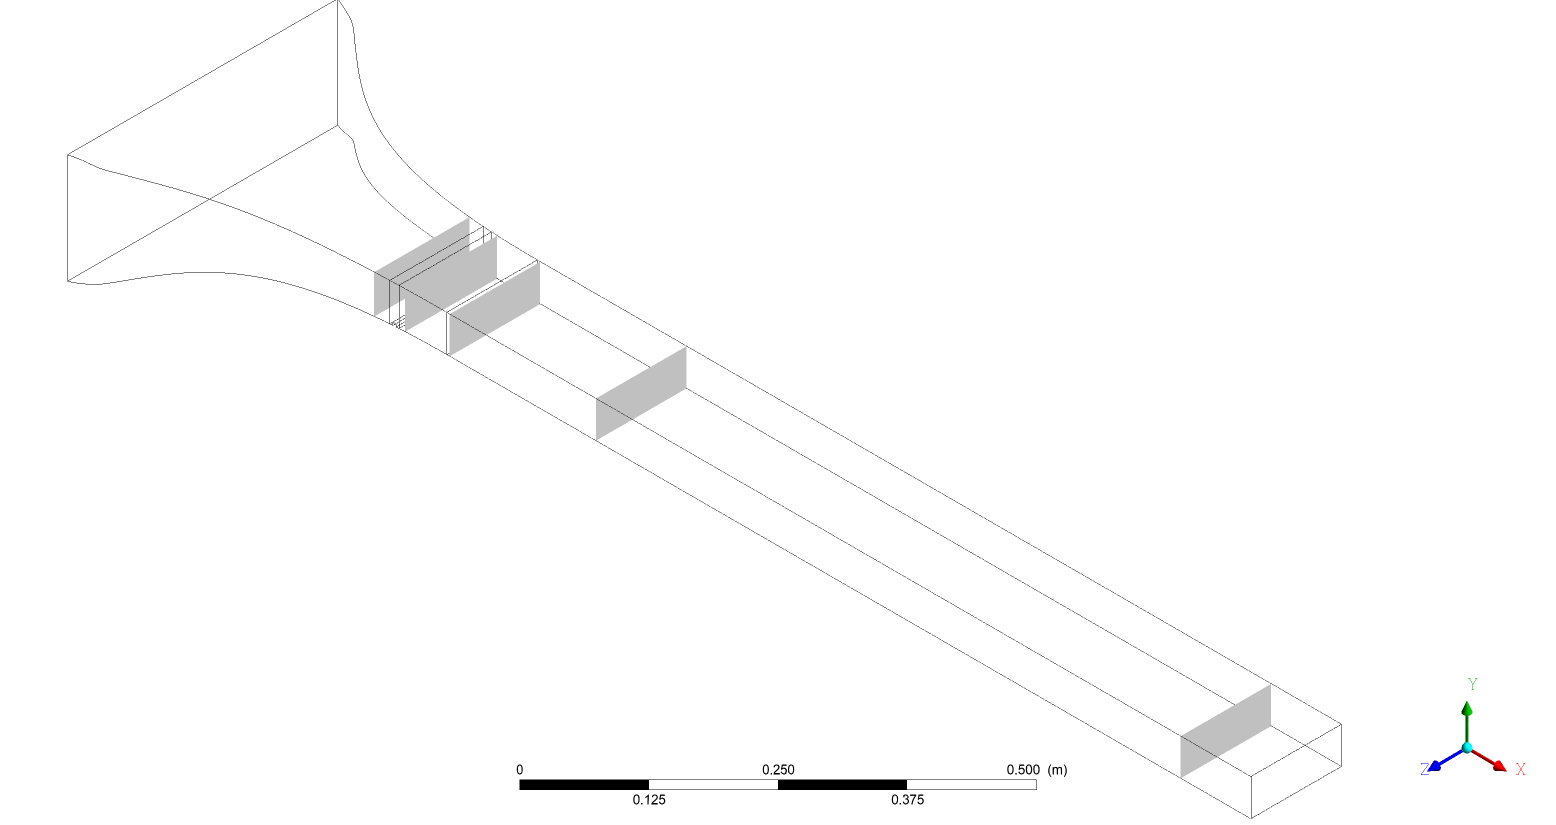
\includegraphics[width=0.9\linewidth]{../Assets/1}
		\caption{Sections for analysis}
		\label{fig:planesforanalysis}
	\end{figure}
	
	The origin of the coordinate axes of the model is located in the center of the channel entrance. Sections were considered at different heights along and at different distances from the entrance to the channel. The table below shows a list of sections, their location and description. Images in applications have names based on the table.
	\begin{table}[H]
		\begin{center}
			\begin{tabular}{|c|c|c|c|}
				\hline
				Label & Plane & Position & Description\\
				\hline
				PlaneXY & XY & Z = 0 & along the whole channel\\
				\hline
				PlaneYZ300 & YZ & X = 300 & in front of the barrier\\
				\hline
				PlaneYZ340 & YZ & X = 340 & after the barrier\\
				\hline
				PlaneYZ400 & YZ & X = 400 & begin of the straight section\\
				\hline
				PlaneYZ600 & YZ & X = 600 & further down the channel\\
				\hline
				PlaneYZ1400 & YZ & X = 1400 & at the exit of the channel\\
				\hline
				PlaneXZ0 & XZ & Y = 0 & above the boundary layer\\
				\hline
				PlaneXZ20M & XZ & Y = -20 & above the barrier\\
				\hline
				PlaneXZ23М & XZ & Y = -23 & at the barrier level\\
				\hline
			\end{tabular}
		\end{center}
		\label{tbl:sections}
		\caption{List of sections}
	\end{table}
	
	After the completion of the calculations, a graph was automatically generated, thanks to which it is possible to evaluate the accuracy of the results obtained on this grid model. It reached a value of $10^{-3}$.
	\begin{figure}[H]
		\centering
		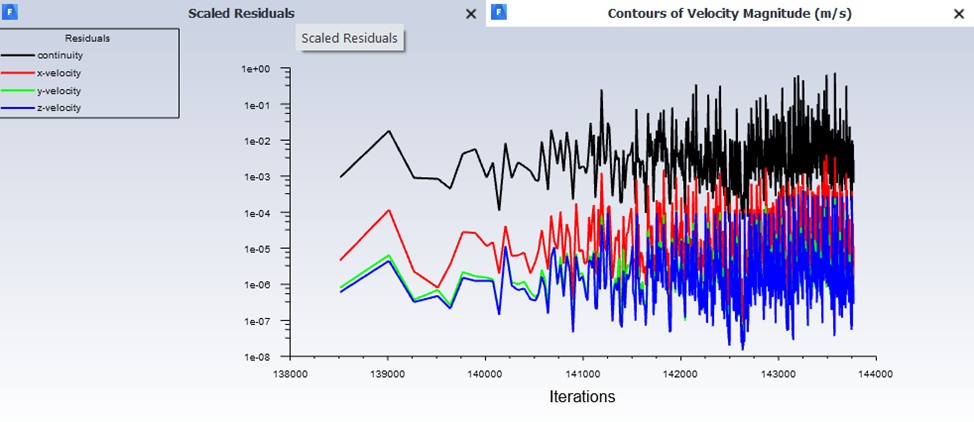
\includegraphics[width=1\linewidth]{../Assets/scaledResiduals}
		\caption{Scaled residuals}
		\label{fig:scaledresiduals}
	\end{figure}
\subsection{Influence on local friction and transport}
	Further, for the convenience of describing the results and their evaluation, several points are presented on various parameters.
\subsubsection{Velocity}
	Let's start with velocity. According to the obtained sections, the contours of average velocity were constructed for various time intervals.
	\begin{figure}[H]
		\centering
		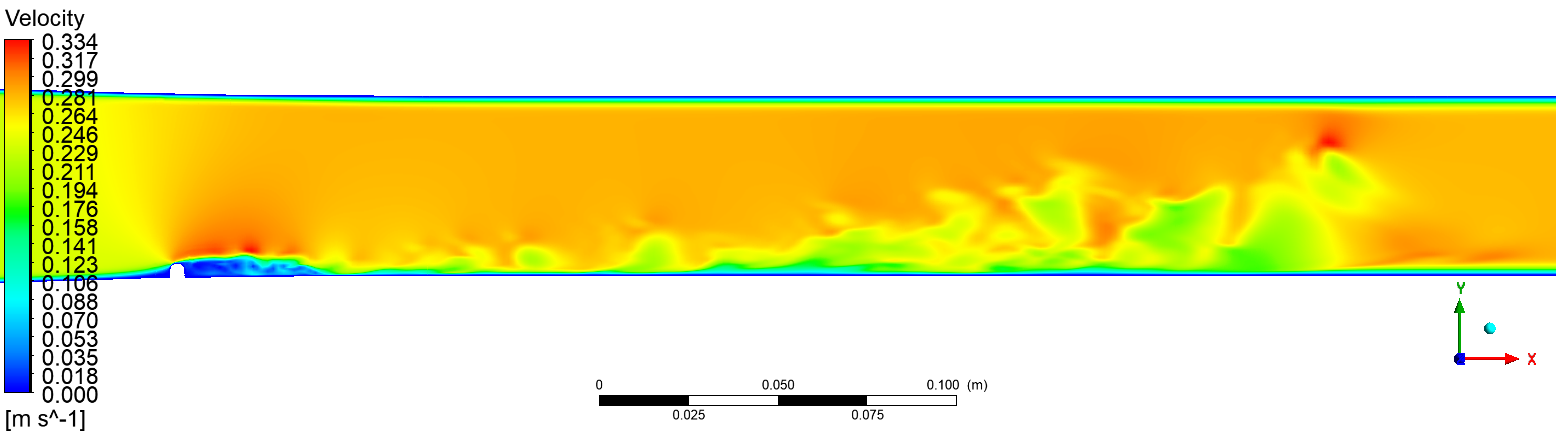
\includegraphics[width=1\linewidth]{../Assets/T16_Velocity_ContourXY}
		\caption{Velocity in longitudinal section XY, t = 1.6 c}
		\label{fig:t16velocitycontourxy}
	\end{figure}
	As can be seen from the figure along the channel, the velocity immediately behind the obstacle and at its level approached zero. And over the wire has increased significantly. Due to such abrupt changes in speed, vortex structures are formed, the speed of which is clearly visible in these images.
	
	\begin{figure}[H]
		\begin{subfigure}{.5\textwidth}
			\centering
			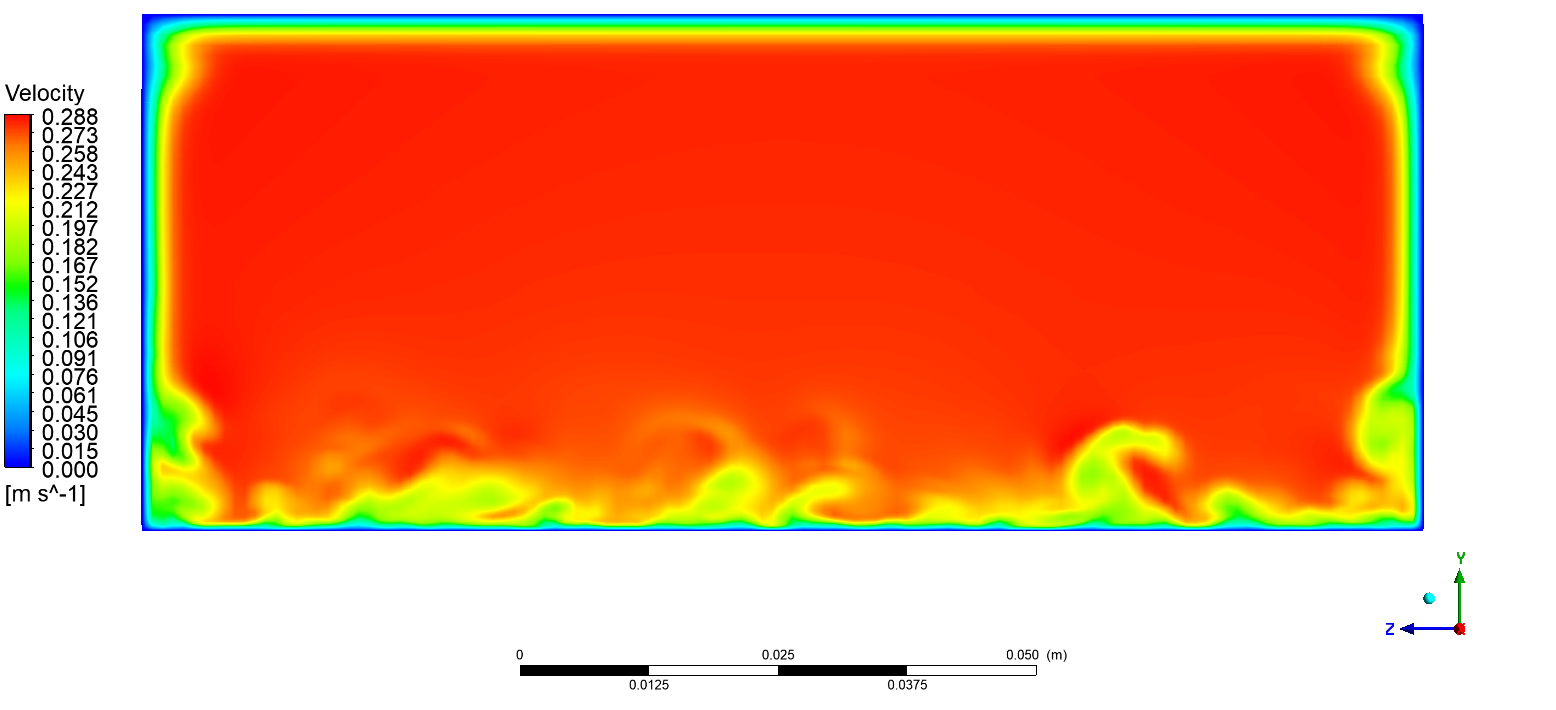
\includegraphics[width=1.1\linewidth]{../Assets/T16_Velocity_ContourYZ400}
			\caption{PlaneYZ400}
			\label{fig:T16VelocityContourYZ340}
		\end{subfigure}%
		\begin{subfigure}{.5\textwidth}
			\centering
			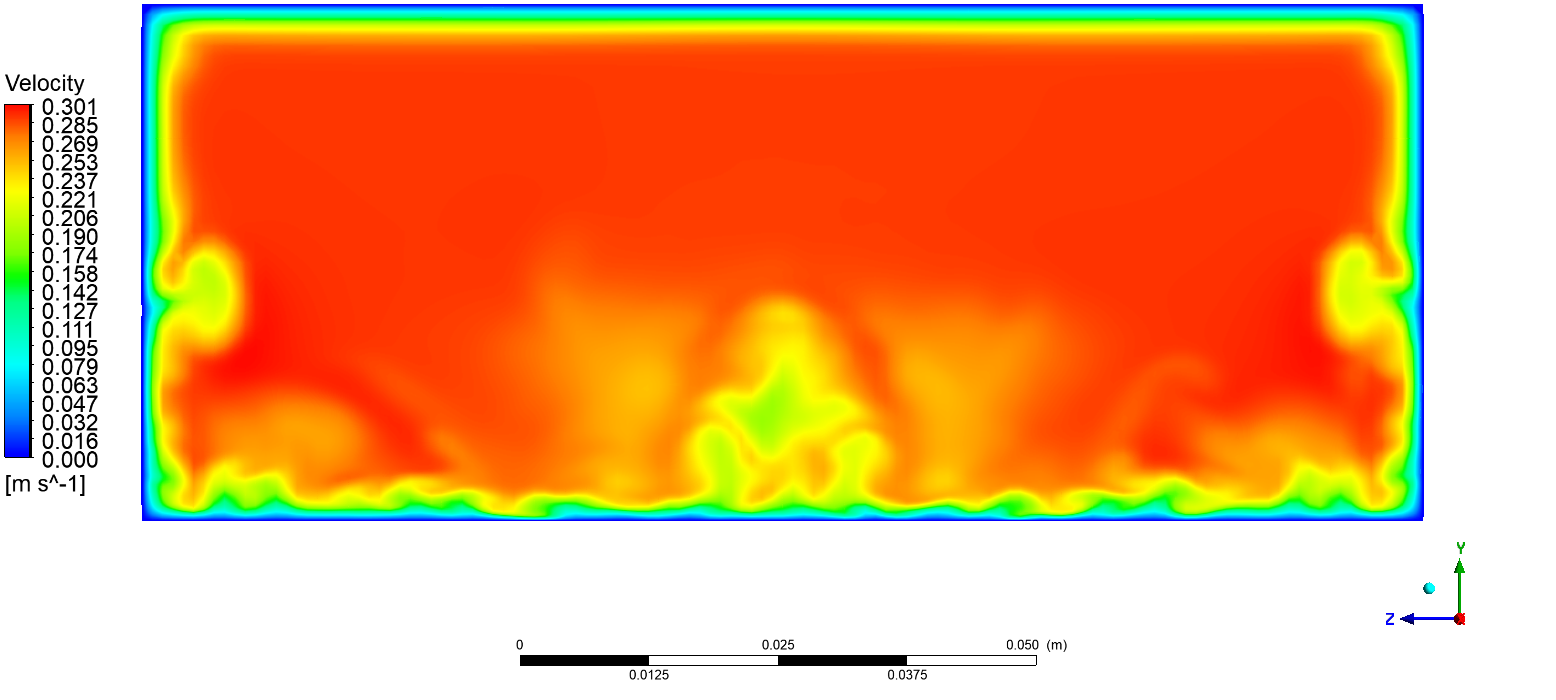
\includegraphics[width=1.1\linewidth]{../Assets/T16_Velocity_ContourYZ600}
			\caption{PlaneYZ600}
			\label{fig:T16VelocityContourYZ400}
		\end{subfigure}
		\caption{Velocity in cross sections at t = 1.6 с}
		\label{fig:T16VelocityContourYZ}
	\end{figure}
	These vortex formations can also be seen in figure \ref{fig:T16VelocityContourYZ}. 
	
	\begin{figure}[H]
		\centering
		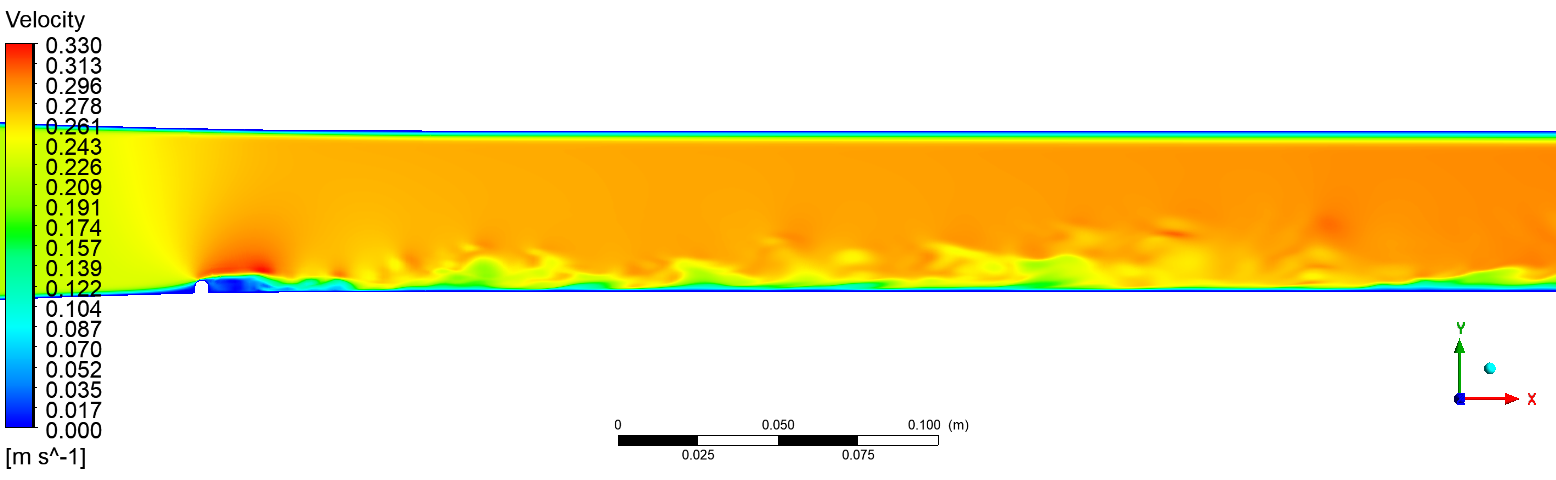
\includegraphics[width=1\linewidth]{../Assets/T96_Velocity_ContourXY}
		\caption{Longitudinal velocity in XY, t = 9.6 с}
		\label{fig:t96velocitycontourxy}
	\end{figure}
	By the time t = 9.6 s, the vortex structure of the channel became less visible and large eddies were transformed into small ones.
	Let us consider more detail velocity in cross sections at time t = 9.6 s.
	\begin{figure}[H]
		\begin{subfigure}{.5\textwidth}
			\centering
			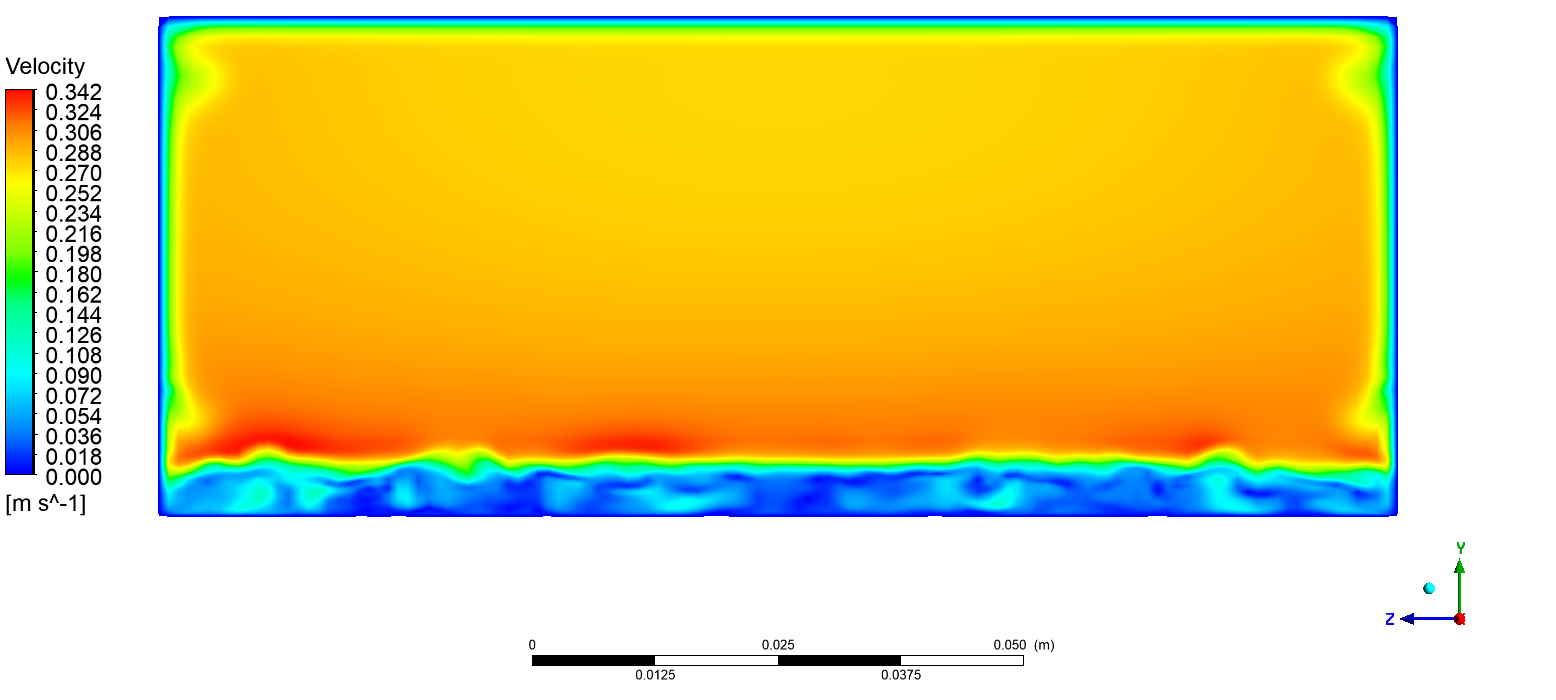
\includegraphics[width=1.1\linewidth]{../Assets/T96_Velocity_ContourYZ340}
			\caption{PlaneYZ340}
			\label{fig:T96VelocityContourYZ340}
		\end{subfigure}%
		\begin{subfigure}{.5\textwidth}
			\centering
			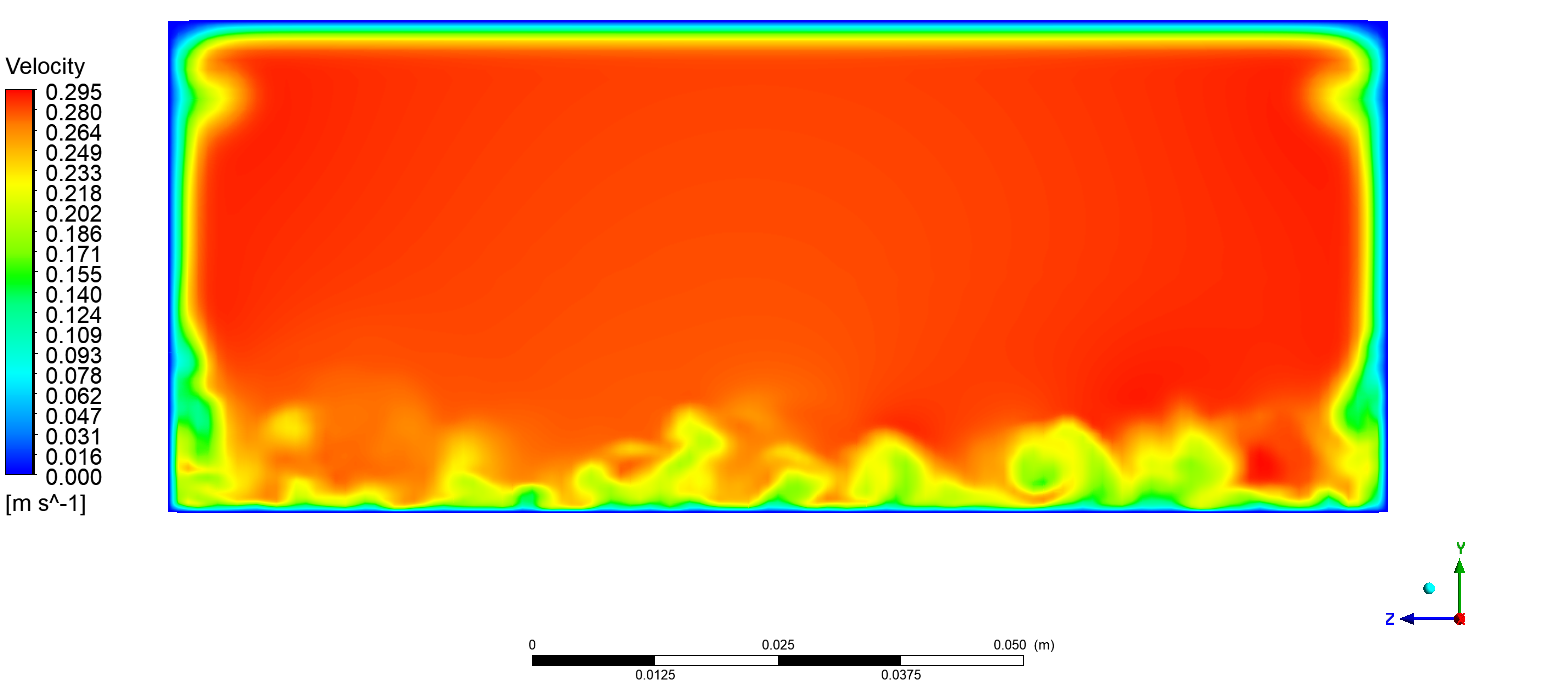
\includegraphics[width=1.1\linewidth]{../Assets/T96_Velocity_ContourYZ400}
			\caption{PlaneYZ400}
			\label{fig:T96VelocityContourYZ400}
		\end{subfigure}
		\\
		\begin{subfigure}{.5\textwidth}
			\centering
			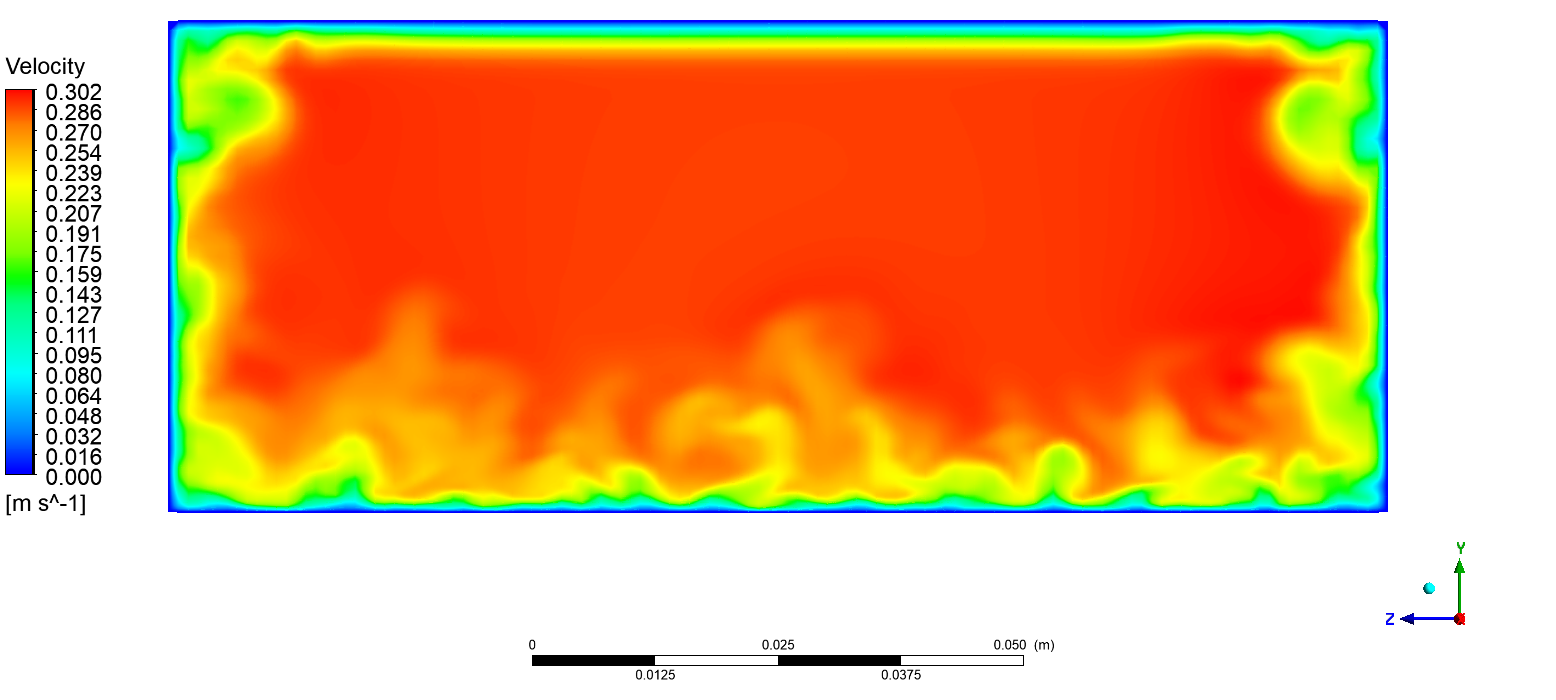
\includegraphics[width=1.1\linewidth]{../Assets/T96_Velocity_ContourYZ600}
			\caption{PlaneYZ600}
			\label{fig:T96VelocityContourYZ600}
		\end{subfigure}%
		\begin{subfigure}{.5\textwidth}
			\centering
			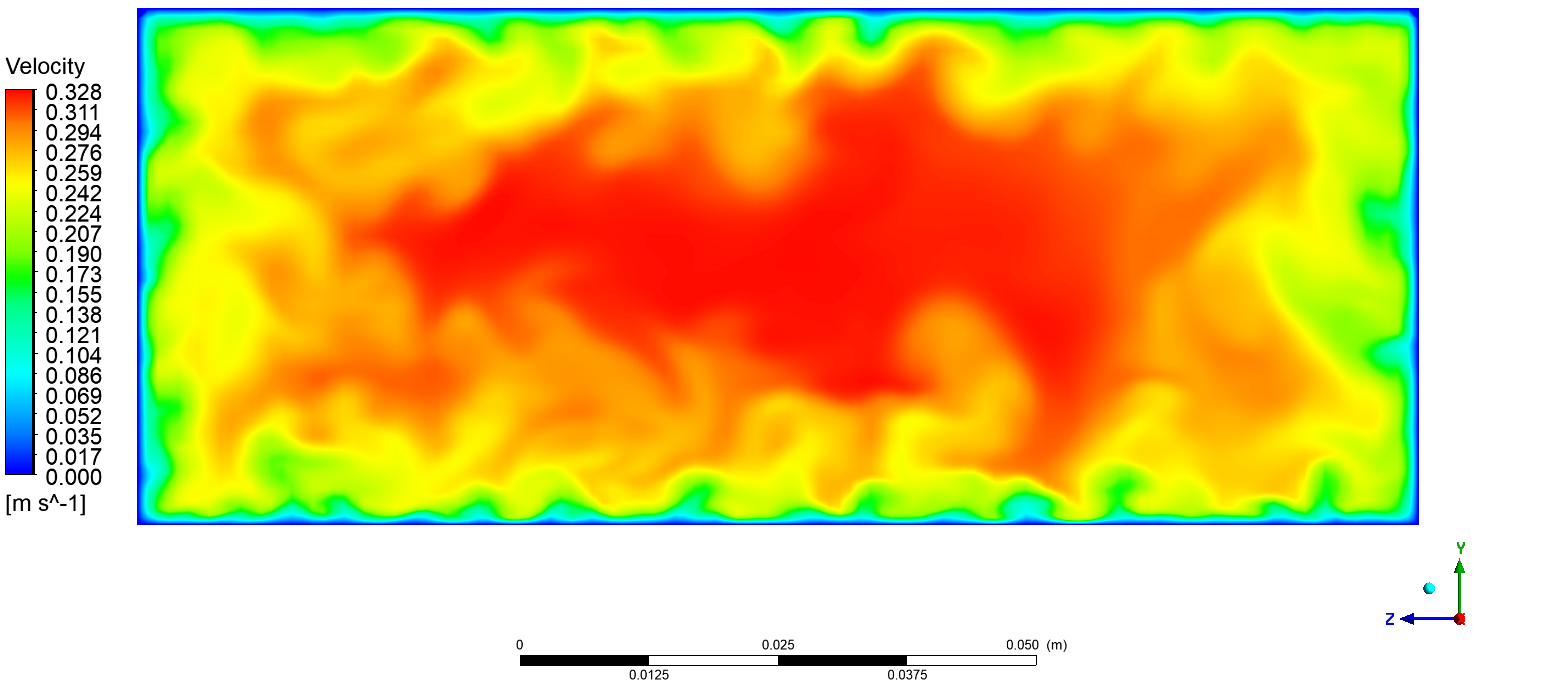
\includegraphics[width=1.1\linewidth]{../Assets/T96_Velocity_ContourYZ1400}
			\caption{PlaneYZ1400}
			\label{fig:T96VelocityContourYZ1400}
		\end{subfigure}
		\caption{Velocity in cross sections at t = 9.6 с}
		\label{fig:T96VelocityContourYZ}
	\end{figure}
	As seen in the picture \ref{fig:T96VelocityContourYZ} the formed vortices gradually decay to Kolmagorov scale vortices and dissipate into energy.
	
	\begin{figure}[H]
		\begin{subfigure}{1\textwidth}
			\centering
			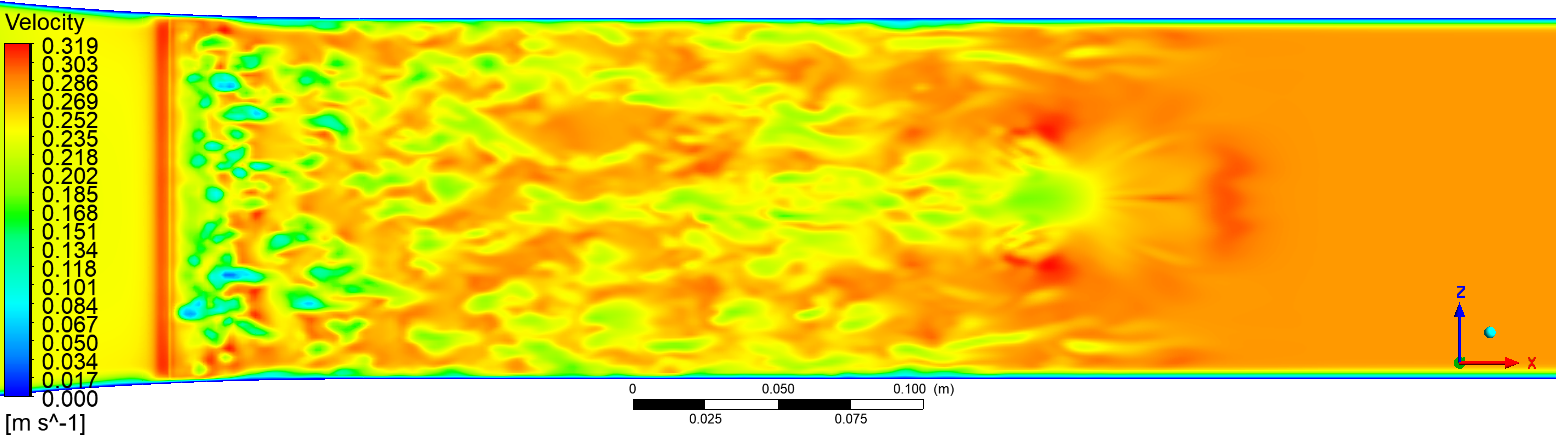
\includegraphics[width=1\linewidth]{../Assets/T16_Velocity_ContourXZ20M}
			\caption{PlaneXZ20M}
			\label{fig:T16VelocityContourXZ20M}
		\end{subfigure}%
		\\
		\begin{subfigure}{1\textwidth}
			\centering
			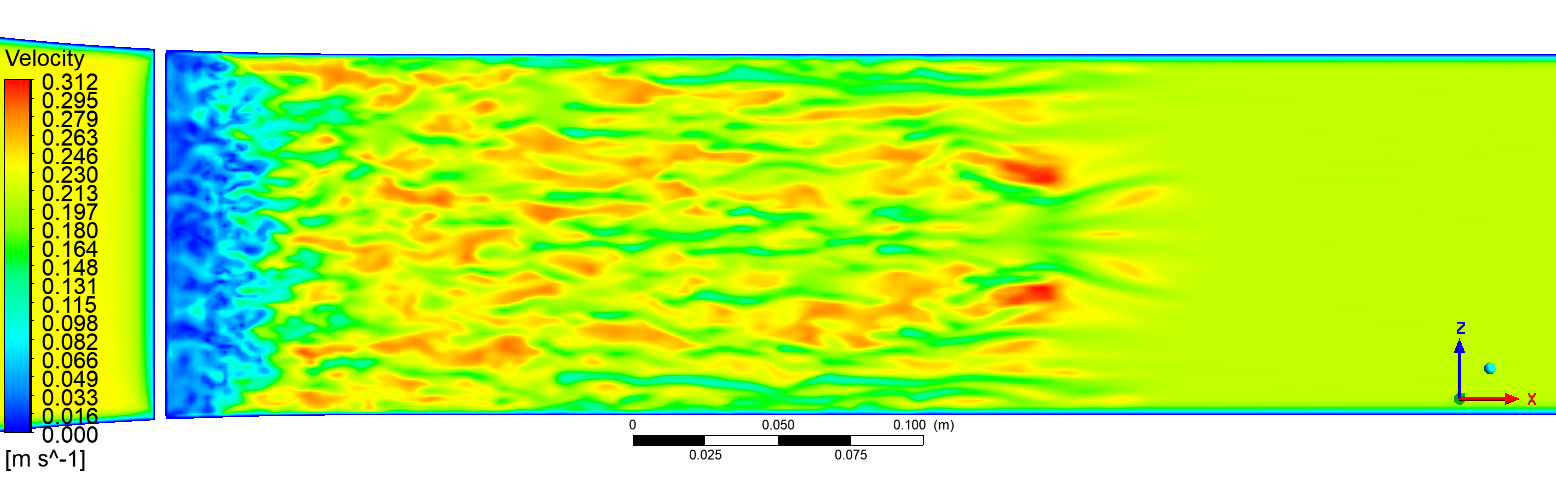
\includegraphics[width=1\linewidth]{../Assets/T16_Velocity_ContourXZ23M}
			\caption{PlaneXZ23M}
			\label{fig:T16VelocityContourXZ23M}
		\end{subfigure}
		\caption{Speed in longitudinal sections XZ at t = 1.6 с}
		\label{fig:T16VelocityContourXZ}
	\end{figure}
\subsubsection{Friction coefficient}
	In order to obtain friction coefficient data for plotting, the necessary sections were built in Ansys Fluent. They divide the channel lengthwise into 3 parts ($z_1 = -31, z_2 = 0, z_3 = 31$). After that, the built-in tools exported the data to $.csv$ files. Further, with the help of MS Excel, the data concerning the boundary layer were selected. And finally, plots are generated in gnuplot. 
	Four time periods were evaluated. The plots show the dependence of $C_f$ on the coordinate $x$. When the fluid flow reaches an obstacle, $C_f$ changes abruptly. The coefficient increased by 2.6 times. As we moved along the length of the channel, the coefficient decreased and stabilized. This is due to a decrease in the influence of vortex structures on the boundary layer.
	\begin{figure}[H]
		\begin{subfigure}{.5\textwidth}
			\centering
			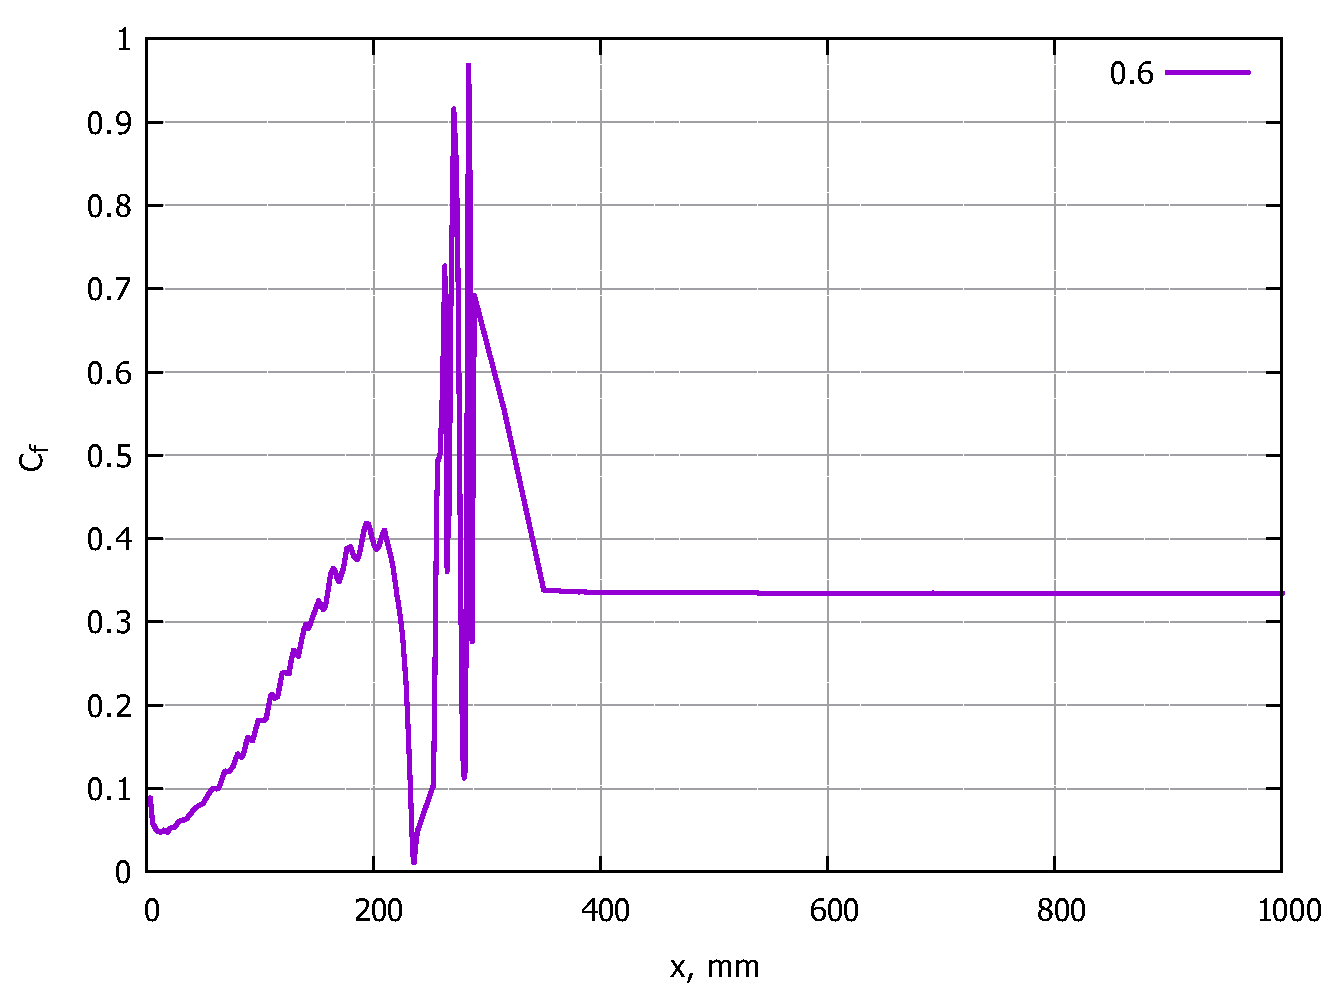
\includegraphics[width=1\linewidth]{../Assets/Cf-T06}
			\caption{t = 0.6 с}
			\label{fig:Cf-T06}
		\end{subfigure}%
		\begin{subfigure}{.5\textwidth}
			\centering
			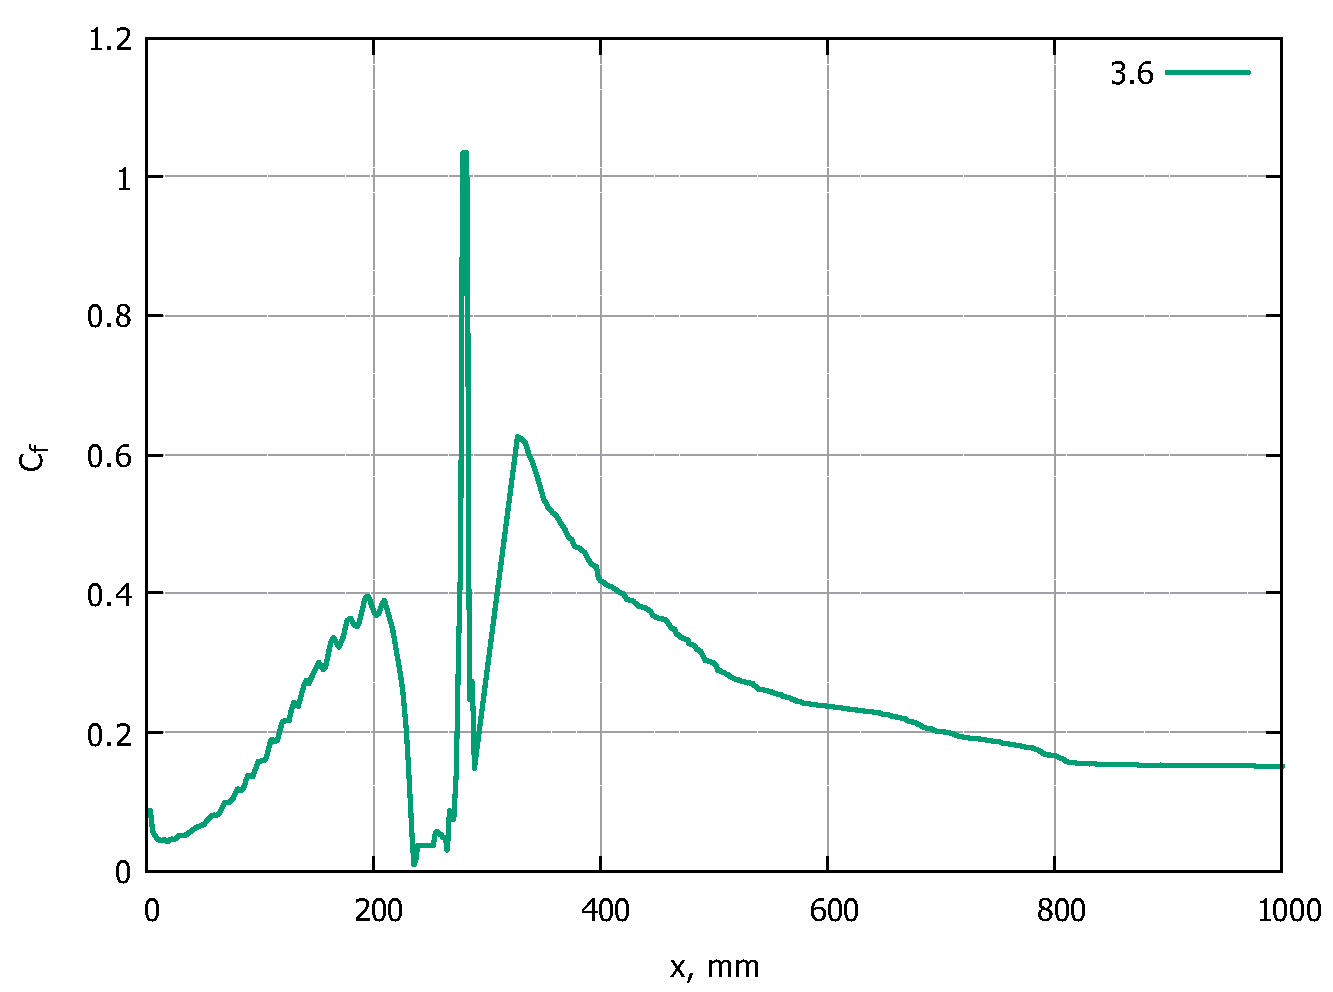
\includegraphics[width=1\linewidth]{../Assets/Cf-T360}
			\caption{t = 3.6 с}
			\label{fig:Cf-T360}
		\end{subfigure}
		\\
		\begin{subfigure}{.5\textwidth}
			\centering
			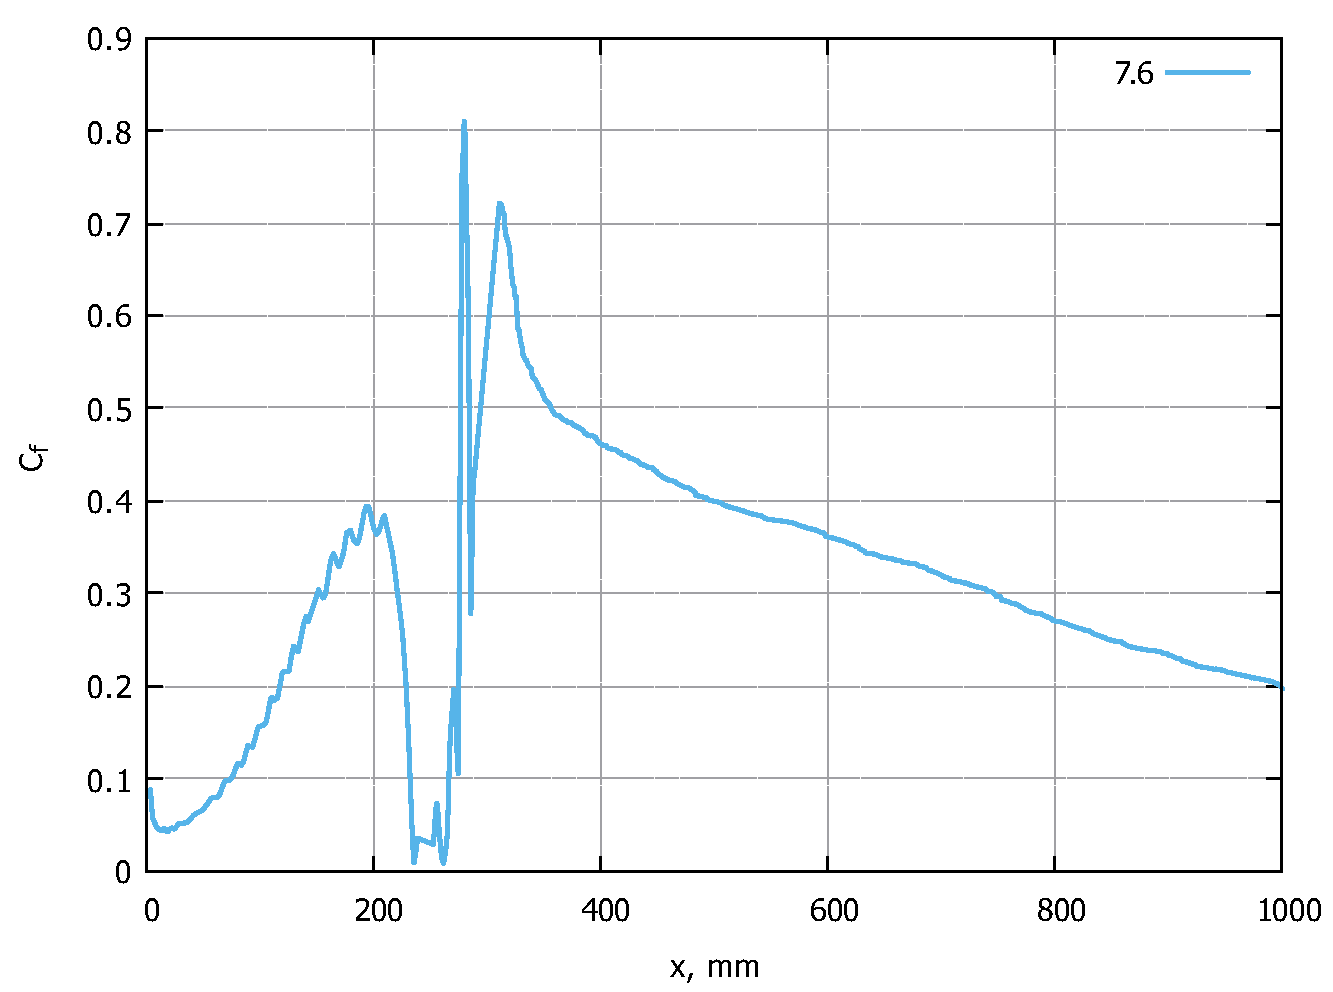
\includegraphics[width=1\linewidth]{../Assets/Cf-T760}
			\caption{t = 7.6 с}
			\label{fig:Cf-T760}
		\end{subfigure}%
		\begin{subfigure}{.5\textwidth}
			\centering
			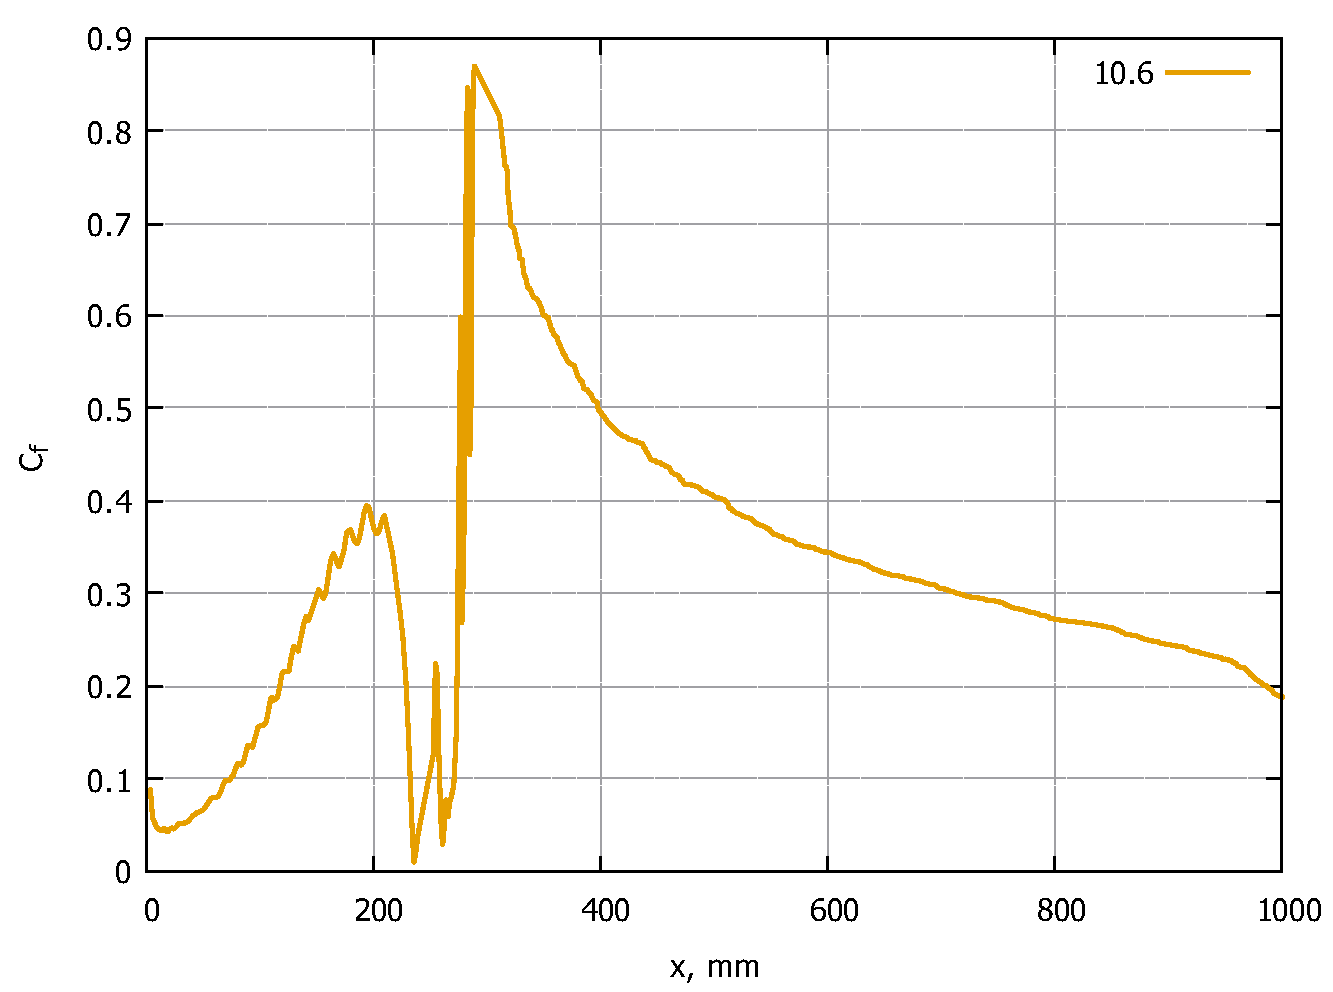
\includegraphics[width=1\linewidth]{../Assets/Cf-T1060}
			\caption{t = 10.6 с}
			\label{fig:Cf-T1060}
		\end{subfigure}
		\caption{Change in the friction coefficient along the length of the channel, z = 0}
		\label{fig:cf}
	\end{figure}
\subsubsection{Q-criterion}
	There are various approaches to the visualization of vortex flows that use one or another definition of a vortex and criteria for its identification. The classification of visualization methods for vortex flows is carried out depending on how the vortex is defined (in the area or on the line), whether the method is invariant with respect to the transformation of the coordinate system, whether the approach is local or global\cite{Hunt1988}. One of these is the $Q$-criterion. It is determined by two components: the strain rate tensor $S$ and the rotation tensor $\Omega$.
	\begin{equation}
		S = \frac{1}{2}(\frac{\partial u_i}{\partial x_j} + \frac{\partial u_j}{\partial x_i}) \qquad \Omega = \frac{1}{2}(\frac{\partial u_i}{\partial x_j} - \frac{\partial u_j}{\partial x_i})
	\end{equation}
	The $Q$-criterion is defined as the second invariant of the velocity gradient tensor\cite{Wiebel2007}.
	\begin{equation}
		Q = \frac{1}{2}(||\Omega||^2 - ||S||^2)
	\end{equation}
	From this we can see that positive values of $Q$ indicate regions in the flow field where vorticity dominates, and negative values of $Q$ indicate regions where strain rate or viscous stress dominates. In addition, there are various versions of the $Q$ criterion in modified expressions that are used to describe different flow regions\cite{Berdahl1993,Chong1990}.
	
	Various areas of eddy formations are presented below. In the figure \ref{fig:q860-t16}, one can notice a clearly expressed structure of the formed vortex.
	\begin{figure}[H]
		\centering
		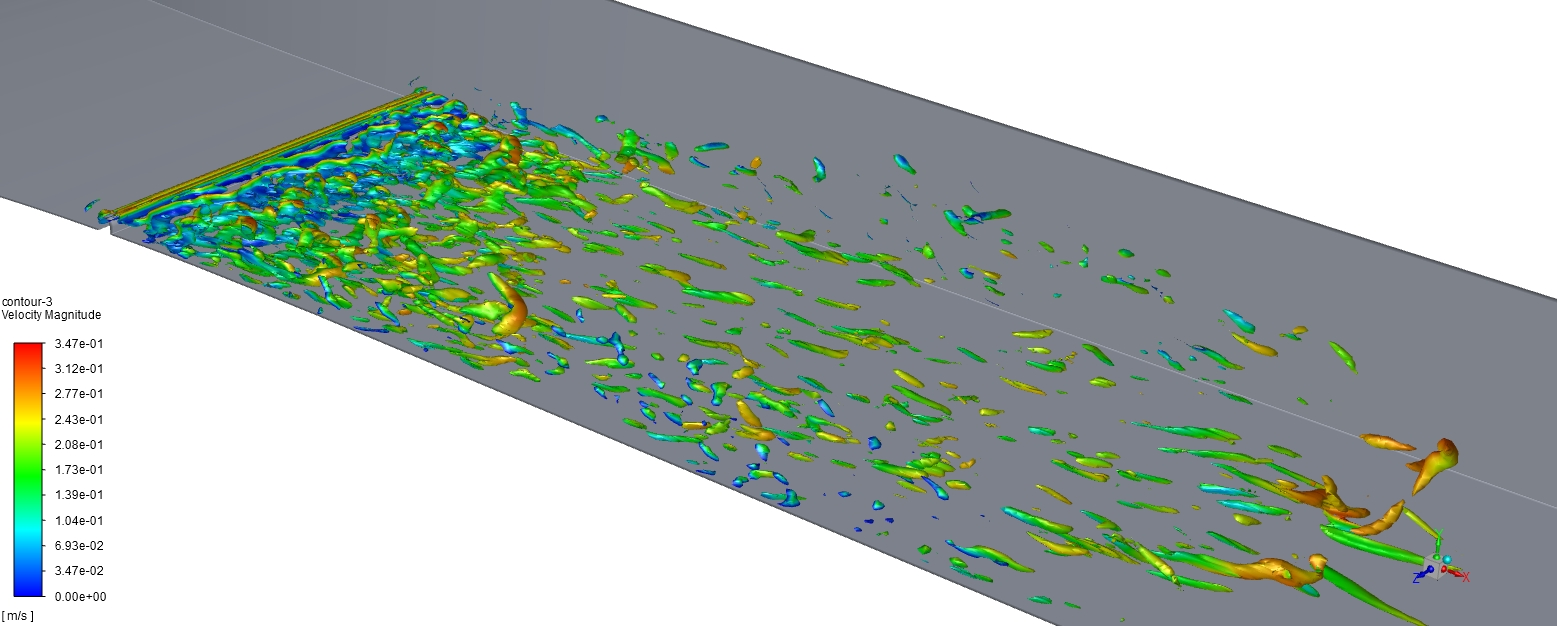
\includegraphics[width=1\linewidth]{../Assets/Q860-t16}
		\caption{Vortex structure at Q = 860 и t = 1.6 c}
		\label{fig:q860-t16}
	\end{figure}
	\begin{figure}[H]
		\centering
		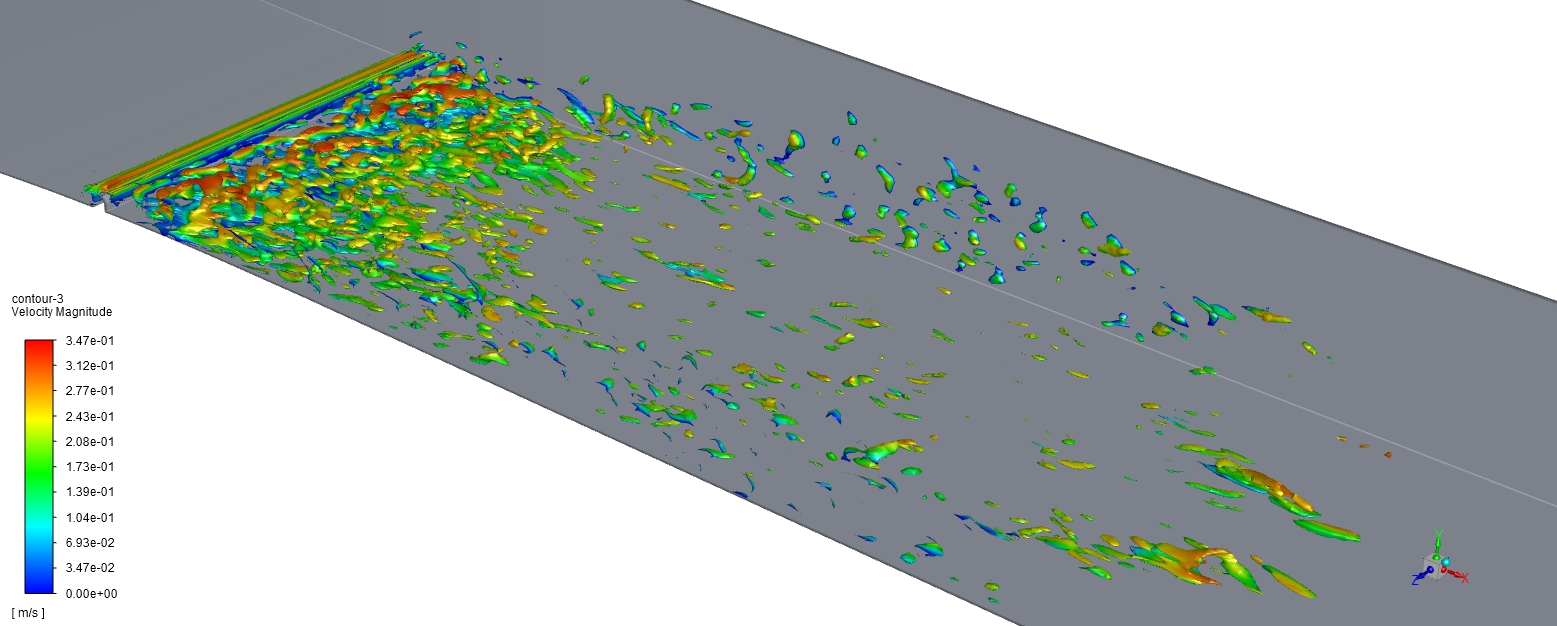
\includegraphics[width=1\linewidth]{../Assets/QM850-t16}
		\caption{Vortex structure at Q = -850 и t = 1.6 с}
		\label{fig:qm850-t16}
	\end{figure}